\documentclass{standalone}
\usepackage{tikz}
\usetikzlibrary{arrows.meta}

\begin{document}
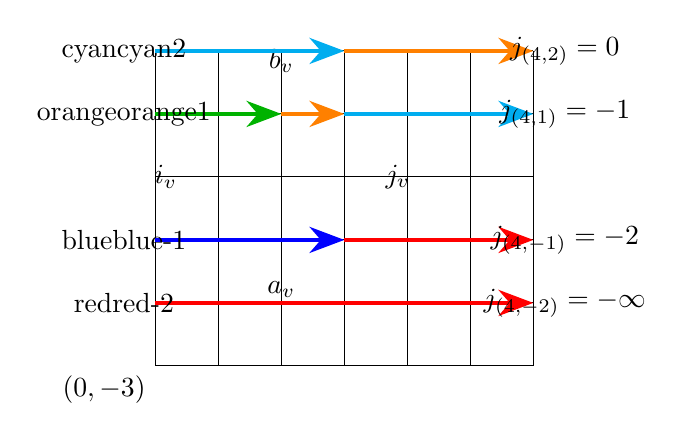
\begin{tikzpicture}[scale=0.8]

% Left diagram: Vertex configuration labels
\draw (-2,0) -- (2,0);
\draw (0,-2) -- (0,2);

\node at (-1.5,0) [left] {$i_v$};
\node at (0,1.5) [above] {$b_v$};
\node at (1.5,0) [right] {$j_v$};
\node at (0,-1.5) [below] {$a_v$};

% Right diagram: Stochastic six-vertex model
\foreach \x in {-2,...,4} {
    \draw (\x,-3) -- (\x,2);
}
\foreach \y in {-3,...,2} {
    \draw (-2,\y) -- (4,\y);
}

% Arrows and colors
\draw[-{Stealth[scale=1.5]},line width=1.2pt,green!70!black] (-2,1) -- (0,1);
\draw[-{Stealth[scale=1.5]},line width=1.2pt,orange] (0,1) -- (1,1);
\draw[-{Stealth[scale=1.5]},line width=1.2pt,cyan] (1,1) -- (4,1);

\draw[-{Stealth[scale=1.5]},line width=1.2pt,cyan] (-2,2) -- (1,2);
\draw[-{Stealth[scale=1.5]},line width=1.2pt,orange] (1,2) -- (4,2);

\draw[-{Stealth[scale=1.5]},line width=1.2pt,blue] (-2,-1) -- (1,-1);
\draw[-{Stealth[scale=1.5]},line width=1.2pt,red] (1,-1) -- (4,-1);

\draw[-{Stealth[scale=1.5]},line width=1.2pt,red] (-2,-2) -- (4,-2);

% Labels for the arrows
\foreach \y/\color/\val in {2/cyan/0, 1/orange/-1, -1/blue/-2, -2/red/-\infty} {
    \node at (-2.5,\y) {\textcolor{\color}{\y}};
    \node at (4.5,\y) {$j_{(4,\y)} = \val$};
}

% Label for the bottom-left corner
\node at (-2,-3) [below left] {$(0,-3)$};

\end{tikzpicture}
\end{document}